\documentclass[12pt]{article}

\usepackage{homeworkpkg}
\usepackage{listings}
\usepackage{minted}
\usepackage{amsmath}
\usepackage{caption}
\usepackage{subcaption}
\PassOptionsToPackage{hyphens}{url}
\usepackage{hyperref}
\usepackage{url}
\usepackage{tikz}
\usetikzlibrary{matrix,chains,positioning,decorations.pathreplacing,arrows,automata}
\usepackage{enumitem}
\setlist{topsep=4pt, itemsep=4pt, partopsep=2pt, parsep=2pt}
\setlength{\parindent}{1.5em}
\setlength{\parskip}{0.5em}

\usepackage{graphicx}
% \usepackage{sourcecodepro}
\usepackage{xcolor}
\definecolor{mizuasagi}{RGB}{102, 186, 183}
\definecolor{kuchiba}{RGB}{226, 148, 59}
\definecolor{sabiseiji}{RGB}{134, 166, 151}
\definecolor{ouchi}{RGB}{155, 144, 194}
\definecolor{dkgreen}{rgb}{0,0.4,0}
\definecolor{gray}{rgb}{0.5,0.5,0.5}
\definecolor{mauve}{rgb}{0.58,0,0.82}
\definecolor{orange}{rgb}{1,0.3,0.15}
\definecolor{codegreen}{rgb}{0,0.6,0}
\definecolor{codegray}{rgb}{0.5,0.5,0.5}
\definecolor{codepurple}{rgb}{0.58,0,0.82}
\definecolor{backcolour}{rgb}{0.96,0.97,0.98}
\lstdefinestyle{mystyle}{
  backgroundcolor=\color{white},
  commentstyle=\color{sabiseiji},
  keywordstyle=\color{dkgreen},
  numberstyle=\tiny\color{codegray},
  stringstyle=\color{kuchiba},
  basicstyle={\footnotesize\ttfamily},
  breakatwhitespace=false,
  breaklines=true,
  captionpos=b,
  keepspaces=true,                 
  numbers=none,                    
  numbersep=5pt,                  
  showspaces=false,                
  showstringspaces=false,
  showtabs=false,                  
  tabsize=2
}
\lstset{style=mystyle}
\lstset{language=python}

\newcommand{\red}[1]{\color{red}{#1}}

%% Local Macros and packages: add any of your own definitions here.

\begin{document}

% Homework number, your name and NetID, and optionally, the names/NetIDs of anyone you collaborated with. If you did not collaborate with anybody, leave the last parameter empty.
\homework
    {}
    {}
    {}
\vspace{-16pt}

\section*{Question 1: K-Means Clustering \pts{20}}

\begin{enumerate}
    \item \textbf{Clustering concepts} \pts{5}
    \par
    \begin{enumerate}
        \item Clustering does not require prior labeling, thus it is a kind of unsupervised learning. Please answer True or False. \pts{1}\\
        \item The goal of all clustering algorithms is to minimize the total within-cluster SSEs (sum of squared error). Please answer True or False and explain your answer. \pts{2}\\
        \item It is impossible to define similarity in terms of clustering for categorical data. Please answer True or False and explain your answer. \pts{2}\\
    \paragraph{}
    \end{enumerate}
    \item \textbf{Clustering applications} \pts{6}
    \par
    Please list at least \textbf{three real applications} of the clustering algorithm. Each of them should include three to four sentences:
    \begin{enumerate}
        \item a brief description of the application
        \item a reference to support your statement (URL link or title of the articles, etc.)
    \end{enumerate}

    \item \textbf{Visualizing a K-means problem} \pts{4}
    \par
    This part of the question aims to help you build an intuitive sense of how the ``K-means algorithm'' works. The following data points are randomly generated with a pre-set number of centroids. 
    \par
    In the following diagrams, try to circle out clusters according to the given $K$ in each of them and then comment on the results. Give your best guess on what should be the optimal $K$, and explain the reason using the ``SSE vs K'' diagram. (Discussed in the Lecture and please refer to Figure 2. For example: if ``K=1'', you should circle all data points to be the same cluster since there is only 1 cluster.)
\begin{figure}[!h]
     \centering
     \begin{subfigure}[b]{0.25\textwidth}
         \centering
         \includegraphics[width=\textwidth]{fig/hw2_q1.png}
         \caption{$K=2$}
         \label{fig:K2}
     \end{subfigure}
     \begin{subfigure}[b]{0.25\textwidth}
         \centering
         \includegraphics[width=\textwidth]{fig/hw2_q1.png}
         \caption{$K=3$}
         \label{fig:K3}
     \end{subfigure}
     \begin{subfigure}[b]{0.25\textwidth}
         \centering
         \includegraphics[width=\textwidth]{fig/hw2_q1.png}
         \caption{$K=4$}
         \label{fig:K4}
     \end{subfigure}
        \label{fig:three graphs}
\vfill
     \centering
     \begin{subfigure}[d]{0.25\textwidth}
         \centering
         \includegraphics[width=\textwidth]{fig/hw2_q1.png}
         \caption{$K=5$}
         \label{fig:K5}
     \end{subfigure}
     \begin{subfigure}[e]{0.25\textwidth}
         \centering
         \includegraphics[width=\textwidth]{fig/hw2_q1.png}
         \caption{$K=6$}
         \label{fig:K6}
     \end{subfigure}
     \begin{subfigure}[f]{0.25\textwidth}
         \centering
         \includegraphics[width=\textwidth]{fig/hw2_q1.png}
         \caption{$K=7$}
         \label{fig:K7}
     \end{subfigure}
        \label{fig:three graphs}
\end{figure}

\begin{figure}[!h]
    \centering
    \includegraphics[width=0.5\textwidth]{fig/hw2_q1_a.png}
    \caption{SSE v.s Number of K}
    \label{fig:my_label}
\end{figure}

    \item \textbf{Calculating and minimizing SSE} \pts{5}
    In this question, calculate the within-cluster SSE with the given information. You should first find out the centroid that minimizes the SSE (We're using Euclidean distance). Please refer to Figure~\ref{fig:hw2_q1_4}.
    \begin{center}
        $A (1, 1)$ \\
        $B (3, 3) $ \\
        $C (5, 1)$ \\
        $D (9, 2)$
    \end{center}
    \begin{figure}[!h]
        \centering
        \includegraphics[width=0.8\textwidth]{fig/hw2_q1_b.png}
        \caption{Points Within a Cluster}
        \label{fig:hw2_q1_4}
    \end{figure}
    
    The detection of outliers (points that should be put into another cluster) is another challenge in clustering problems, and a naive way to identify the outlier is to remove one of the points and then observe the change of within-cluster SSE. Repeat this step until the outlier that leads to the largest drop in SSE is confirmed.
    
    Assume we know there is an outlier in the given cluster, identify it, and calculate the new minimum within-cluster SSE. Then, explain why you choose this point as the outlier.

\end{enumerate}

\newpage
\section*{Question 2: Linear Classifiers, SVM and Mapping Trick \pts{21}}
\begin{enumerate}
    \item \textbf{Linear Classifiers} \pts{4}\\
    Consider two classification problems in a 2D space:
    \begin{enumerate}
        \item Data points belonging to label \texttt{‘0’}: \{(0,0), (0,1)\}.\\ Data points belonging to label \texttt{‘1’}: \{(1,0), (1,1)\}.
        \item Data points belonging to label \texttt{‘0’}: \{(0,0), (1,1)\}.\\ Data points belonging to label \texttt{‘1’}: \{(1,0), (0,1)\}.
    \end{enumerate}
    Can linear classifiers learn each pattern in these two classification problems? Justify your answer.

    \item \textbf{1-D Linear Classification} \pts{5}\\
    To demonstrate the mapping trick as we discussed in the lecture, we first consider a 1D classification problem.  Suppose that we have the following points to be classified:
    \begin{center}
        Class A: (-2, -1.8, 0.3, 0.6, 1)  Label: -1\\
        Class B: (-1, -0.7, -0.6, -0.3, 2) Label: 1\\
    \end{center}
    Plot the points on a number axis, and comment on whether they can be perfectly classified with a 1D linear classifier.\\
    Hint: a linear classifier in 1D can be seen as assigning different labels to $x>b$ and $x<b$ where $b$ is the division (hyperplane).\\
    
    \item \textbf{The Mapping Trick} \pts{6}\\
    Now, transform the points into a 2D space using the following mapping function:
    \begin{align*}
        \psi(x) = (x, x^3-2x)
    \end{align*}
    \par Again, plot the points in a 2D coordinate system and comment on whether they can be classified with a simple linear classifier and explain why or why not. Make sure the scales of your x-axis and y-axis are the same; it will make your next questions much easier.\\
    
    \item \textbf{SVM and hyperplane} \pts{6}\\
    Based on the plot that you have obtained from the previous questions, follow the steps below and find the hyperplane for the SVM. (You don't need to solve for the line algebraically. )
    \begin{enumerate}
        \item What is the geometric interpretation of the hyperplane in SVM?\\
        
        \item Circle the point in each class that is the closest to the other class. What is the relationship between these two points and the hyperplane?\\
        
        \item Based on the above relationship, describe how to find the hyperplane (which should simply be a straight line) and draw it in the plot.  
    \end{enumerate}
\end{enumerate}

\newpage
\section*{Question 3: Neural Network Basics \pts{20}}
\begin{enumerate}
    \item For a classification problem with 16 input features and 16 classes, compare the following two networks:
    \begin{enumerate}
        \item a deeper network with nine dense (fully connected) layers with 32 nodes in each layer
        \item a shallower network that has three dense (fully connected) layers with 128 nodes in each layer
    \end{enumerate} 
    If we use \texttt{float32} to store the weights, what are the memory requirements of these two configurations? Which one would you prefer to deploy on an edge device? (The networks have no bias. 32 bits is 4 bytes. The network in Slide 4 of Lecture 9 has four fully connected layers.) \pts{4}\\
    Hint: The input layer is not included in the above configuration. \\
    
    \item You have trained a DNN model for static image classification applications. You deploy the model in the field with a camera. However, you find that the camera’s view has shifted in space compared to the camera used for capturing training images. In other words, the area of interest has moved off-center while the objects in your training images are perfectly at the center. What would happen to the classification accuracy if you used (1) a Multi-layer Perceptron or (2) a Convolutional Neural Network as your model? Justify your answer (Think about Translation Invariance). \\What would happen to the performance of the model if you add max pooling layers into CNN in this scenario? \pts{3}\\
    
    \item Batch normalization layers are used in most of today’s state-of-the-art convolutional neural networks. We can \textit{fuse} the batch normalization layer into the convolutional layer. Suppose we have $w_i$ and $b_i$ to denote the weight and bias in the convolutional layer. Write down the new $w_i'$ and $b_i'$ for the fused convolutional layer with the parameters from the batch normalization. \pts{4}\\

    \item You are building a classifier and considering three different activation functions: ReLU, tanh, and unit step function.
    \begin{enumerate}
       \item Please sketch the three activation functions. \pts{3}\\
       \item Which one is the most popular of the three? Name two advantages of this activation function over the other two. \pts{2}\\
    \end{enumerate}
    
    \item Assuming your design needs to fetch $N$ weights from the memory and the average memory access bandwidth is $B$ bytes per second, calculate the data transfer latency (in the unit of second) when using FLOAT32 to represent each weight. Then, calculate the data transfer latency if we apply quantization to convert the model to INT8. \pts{4}
    
\end{enumerate}

\newpage
\section*{Question 4: Convolution \pts{16}}
\begin{enumerate}
    \item We want to perform a convolution operation on a feature map. This function takes the feature map and the kernel as inputs and returns the output features. Calculate and fill in the parentheses with proper numbers of the dimensions of the output feature map and loop ranges. Assume there is no padding to the input feature map.\pts{6} \\
\begin{figure}[h!]
\hspace{3em}
\begin{subfigure}[b]{0.8\textwidth}
    \begin{minted}[frame=lines, fontsize=\small, linenos]{python}
def convolution(input_fm, kernel) {
    """
    Inputs:
    - input_fm:   A 3D numpy array of shape 
                    (3, 223, 223).
    - weights:    A 4D numpy array of shape 
                    (16, 3, 3, 3).
    
    Returns:
    - output_fm:  A 3D numpy array of shape 
                    (channel_out, height_out, width_out).
    """

    height_out = (            ) #height of the output feature map
    width_out = (            ) #width of the output feature map
    channel_out = (            ) #channel number of the output feature map

    output_fm = np.zeros((channel_out, height_out, width_out)) 
    #empty feature map in the designated shape
    
    for row in range(            ):
        for col in range(            ):
            for to in range(            ):
                for ti in range(            ):
                    for ki in range(            ):
                        for kj in range(            ):
                            output_fm[to][row][col] += \
        weights[to][ti][ki][kj] * input_fm[ti][row + ki][col + kj]

    return output_fm
}
    \end{minted}
\end{subfigure}
\caption{Q4.1 Stride 1 Convolution}
\end{figure}

\newpage
\item If we wish to perform a stride-2 convolution instead of a stride-1 (unit stride) convolution such as the one above, which numbers will change? Please fill in the new numbers in the blanks below. Again, no padding for the input feature map.\pts{2}

\begin{figure}[h!]
\hspace{3em}
\begin{subfigure}[b]{0.8\textwidth}
    \begin{minted}[frame=lines, fontsize=\small, linenos]{python}
def convolution_s2(input_fm, kernel) {
    """
    Inputs:
    - input_fm:   A 3D numpy array of shape 
                    (3, 223, 223).
    - weights:    A 4D numpy array of shape 
                    (16, 3, 3, 3).
    
    Returns:
    - output_fm:  A 3D numpy array of shape 
                    (channel_out, height_out, width_out).
    """

    height_out = (            )
    output_out = (            )
    channel_out = (            )

    output_fm = np.zeros((channel_out, height_out, width_out))
    
    for row in range(            ):
        for col in range(            ):
            for to in range(            ):
                for ti in range(            ):
                    for ki in range(            ):
                        for kj in range(            ):
                            output_fm[to][row][col] += \
        weights[to][ti][ki][kj] * input_fm[ti][row + ki][col + kj]

    return output_fm
}
    \end{minted}
\end{subfigure}
\caption{Q4.2 Stride 2 Convolution}
\end{figure}

\item Consider the first question with the normal unit-stride convolution; we use that as one layer in our neural network. Please think about the following questions and answer in one to two sentences.
\begin{enumerate}
    \item Can the loops that go through the kernel dimension (ki, kj) be swapped with the ones that go through the output dimensions (row, col) without causing any issues? Explain when it's okay to switch the order of loops and how it might affect the speed and way of accessing memory. \pts{2}\\
    
    \item If you wish to increase the \textbf{receptive field} of your network layer, what do you need to change? \pts{2}\\
    
    \item What is one potential benefit of a larger receptive field? Can a larger receptive field do any harm in practical applications? \pts{2}\\

    \item What is the significance of the output channel and how is the number of output channels determined? Why is it usually larger than the input channel? \pts{2}\\
\end{enumerate}

\end{enumerate}
\newpage
\section*{Question 5: Backpropagation \pts{15}}
Consider a simple neural network in Figure \ref{fig:NNPipe}. Single-circled nodes denote variables: $x_1$ is an input variable, $h_1$ and $h_2$ are intermediate variables (first layer), and $\hat{y}$ is an output variable (second layer), etc. Double-circled nodes denote functions: $\Sigma$ takes the sum of its inputs, and $\sigma$ denotes the logistic function $\sigma(x)=\frac{1}{1+e^{-x}}$.

Suppose we have an MSE (Mean Square Error) loss $L(y,\hat{y})=\lVert y-\hat{y}\rVert^{2}_{2}$, We are given a data point $(x1, x2, x3, x4) = (0.3, 1.4, 0.9, -0.6)$ with the true label 0.37. The gradient of the MSE loss function is $2\lVert y-\hat{y}\rVert$.

\begin{enumerate}
\item First perform forward propagation and compute $s_1, s_2, s_3, h_1, h_2$, and $\hat{y}$. Then, use the backpropagation algorithm introduced in Lecture 8 to compute the partial derivative $\frac{\partial L}{\partial w_1}$,$\frac{\partial L}{\partial w_2}$,$\frac{\partial L}{\partial w_3}$,$\frac{\partial L}{\partial w_4}$,$\frac{\partial L}{\partial w_5}$,$\frac{\partial L}{\partial w_6}$. \pts{12}\\\\
Hint: Remember that during backpropagation, the gradient computed for a later layer can be reused when calculating the gradient for earlier layers. \\

\item Explain vanishing gradients and exploding gradients. You can watch  \href{https://www.youtube.com/watch?v=qhXZsFVxGKo}{\textcolor{dkgreen}{this video}} before answering the question. \pts{3}

\end{enumerate}

\begin{figure}[h!]
    \centering
    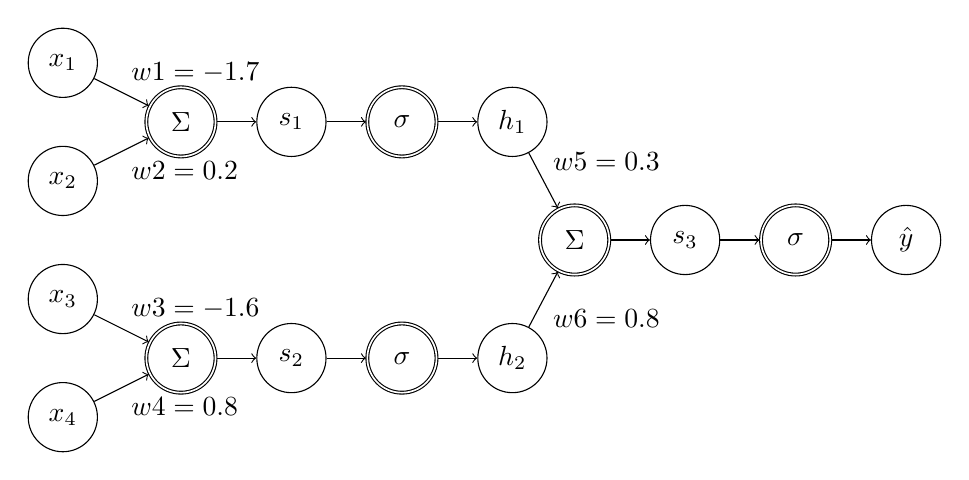
\begin{tikzpicture}[node distance=0.5cm,
        % define styles    
        init/.style={ 
             draw, 
             circle, 
             inner sep=2pt,
             font=\Large,
             join = by -latex
        },
        squa/.style={ 
            font=\Large,
            join = by -latex
        }
    ]
        
        % Top chain x1 to w1
        \begin{scope}[start chain=1]
        \node[on chain=1,state] at (0,1.5cm)  (x1) {$x_1$};
        \end{scope}
        \begin{scope}[start chain=2]
        \node[on chain=2,state,accepting] at (1.5cm,0.75cm) (Sigma1) {$\displaystyle\Sigma$};
        \node[on chain=2,state]  (s1) {$s_1$};
        \node[on chain=2,state,accepting]  (sigma1) {$\displaystyle\sigma$};
        \node[on chain=2,state]  (h1) {$h_1$};
        \end{scope}
        \begin{scope}[start chain=3]
        \node[on chain=3,state] at (0,0cm)  (x2) {$x_2$};
        \end{scope}
        
        \begin{scope}[start chain=4]
        \node[on chain=4,state] at (0,-1.5cm)  (x3) {$x_3$};
        \end{scope}
        
        \begin{scope}[start chain=5]
        \node[on chain=5,state,accepting] at (1.5cm,-2.25cm) (Sigma2) {$\displaystyle\Sigma$};
        \node[on chain=5,state]  (s2) {$s_2$};
        \node[on chain=5,state,accepting]  (sigma2) {$\displaystyle\sigma$};
        \node[on chain=5,state]  (h2) {$h_2$};
        \end{scope}
        
        \begin{scope}[start chain=6]
        \node[on chain=6,state] at (0,-3cm)  (x4) {$x_4$};
        \end{scope}
        
        \begin{scope}[start chain=7]
        \node[on chain=7,state,accepting] at (6.5cm,-0.75cm)  (Sigma3) {$\displaystyle\Sigma$};
        \node[on chain=7,state]  (s3) {$s_3$};
        \node[on chain=7,state,accepting]  (sigma3) {$\displaystyle\sigma$};
        \node[on chain=7,state]  (y) {$\hat{y}$};
        
        \end{scope}
        \path[->] (x1) edge [above right ]       node [align=center]  {$ w1 = -1.7 $} (Sigma1)
        (x2) edge [below right ]       node [align=center]  {$ w2 = 0.2 $} (Sigma1)
        (Sigma1) edge (s1)
        (s1) edge (sigma1)
        (sigma1) edge (h1)
        (h1) edge [above right ]       node [align=center]  {$ w5 = 0.3 $}  (Sigma3)
        (Sigma3) edge (s3)
        (s3) edge (sigma3)
        (sigma3) edge (y)
        
        (x3) edge [above right ]       node [align=center]  {$ w3 = -1.6 $} (Sigma2)
        (x4) edge [below right ]       node [align=center]  {$ w4 = 0.8 $} (Sigma2)
        (Sigma2) edge (s2)
        (s2) edge (sigma2)
        (sigma2) edge (h2)
        (h2) edge [below right ]       node [align=center]  {$ w6 = 0.8 $} (Sigma3)
        
        ;
        % Middle chain x2 to output
    \end{tikzpicture}
    \caption{A Simplified Neural Network Example}
    \label{fig:NNPipe}
\end{figure}

\newpage
\section*{Question 6: Find Bugs in Tensorflow Code [8 pts]}

Bob has recently working on Lab 2. He is not satisfied with small datasets such as Fashion MNIST, and he wants to explore more interesting datasets. He decides to build a simple Multi-Layer Perceptron (MLP) classifier using TensorFlow with Keras to classify images from the \href{https://www.cs.toronto.edu/~kriz/cifar.html}{CIFAR-10 dataset}. The CIFAR-10 dataset consists of 60,000 32x32 color images in 10 classes, with 6,000 images per class, which is a cool choice for developing and testing image classification models.

However, Bob is relatively new to TensorFlow and neural network design. He wrote the following code to build, compile, and train his MLP model. However, Bob noticed that his model doesn't work, and he suspects there must be some bugs in his code.

As Bob's helpful friend, you would like to review Bob's code, identify any bugs that might be present, and \textbf{explain} how they could affect the model's performance by making a short comment next to the code. After identifying the bugs, suggest corrections to make the model work. (Hints: There are 4 bugs in the code. For information on possible loss functions, please refer to \href{https://keras.io/api/losses/}{the link}.)


\begin{minted}[frame=lines, fontsize=\small, linenos]{python}
import tensorflow as tf
from tensorflow.keras import layers, models
from tensorflow.keras.datasets import cifar10
from tensorflow.keras.utils import to_categorical

# Load and preprocess the CIFAR-10 dataset as int arrays
(train_images, train_labels), (test_images, test_labels) \
        = cifar10.load_data()
# Normalize the images
train_images, test_images \
        = train_images * 255.0, test_images * 255.0
train_labels, test_labels \
        = to_categorical(train_labels), to_categorical(test_labels)

# Build the MLP model
model = models.Sequential([
    layers.Flatten(input_shape=(32, 32, 1)),
    layers.Dense(512, activation='relu'),
    layers.Dense(256, activation='relu'),
    layers.Dense(10, activation='relu')
])

# Compile the model
model.compile(optimizer='adam',
              loss='binary_crossentropy',
              metrics=['accuracy'])

# Train the model
model.fit(train_images, train_labels, epochs=10, \
        batch_size=64, validation_split=0.2)

# Evaluate the model
test_loss, test_acc = model.evaluate(test_images, test_labels)
print(f'Test accuracy: {test_acc:.3f}')
    \end{minted}

\end{document} 